\chapter{研究方法}
\label{cha:methods}

\section{数据集}

本研究使用的数据集为 \href{https://ipv6hitlist.github.io}{https://ipv6hitlist.github.io} 提供的约 4 亿个 IPv6 地址. 这些地址是为 IPv6 网络扫描相关研究而收集并不断更新的可响应的 IPv6 地址集.

\section{信息熵分析}

信息熵是一种对信息的不可预测性的度量. 其定义为:

$$H(x) = - \sum\limits_{i=1}^{k} P(x_i) \log P(x_i)$$

一般而言, 信息熵越大, X 值的分布就越无序. 当信息熵为 0 时, X 为定值.

信息熵揭示了 IPv6 地址中可变部分与相对不可变部分. 我们提出了一个简单的基于阈值的分割算法, 用于基于信息熵将 IPv6 地址中相邻的半字节合并为一个地址段: 将相邻的半字节划分为一个段, 当相邻半字节信息熵的差超过阈值时开始新的段划分.

图~\ref{fig:entropy}~绘制了样本集每半字节的信息熵. 通过比较相邻半字节的信息熵, 我们将 IPv6 地址划分为若干地址段. 该图用虚线划分地址段, 用大写字母标记. 对于该样本集, 我们将其划分为 A-N 14 个地址段.

\begin{figure}[htbp]
\centering
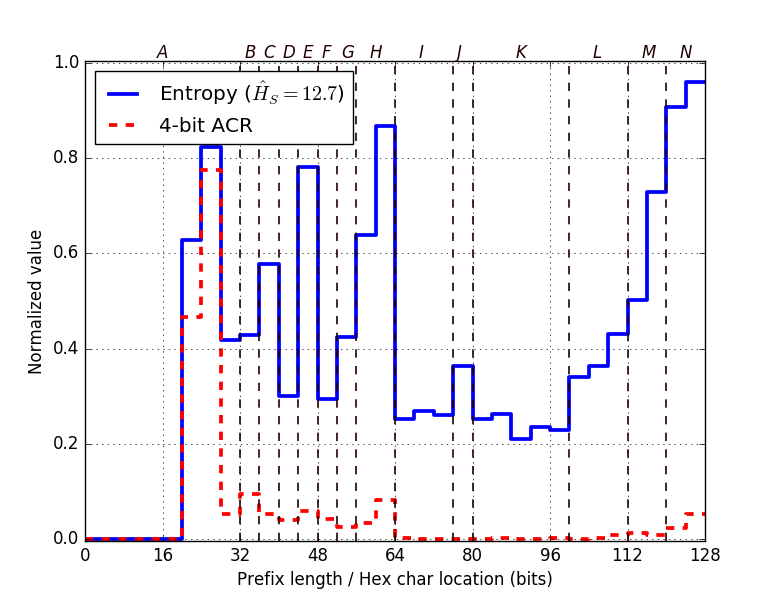
\includegraphics[width=0.5\textwidth]{entropy}
\caption{信息熵}
\label{fig:entropy}
\end{figure}

\section{DBSCAN}

在进一步分析中, 我们想要理解为什么一些值非随机的出现. 我们同时考虑值的频率和值本身, 提出了一个简单的基于阈值的聚类算法: 对每一个段, 首先找出那些出现频率超过阈值的值, 然后用基于密度的聚类算法 DBSCAN 对余下的值进行聚类.

图~\ref{fig:dbscan}~展示了部分样本集的聚类结果.

\begin{figure}[htbp]
\centering
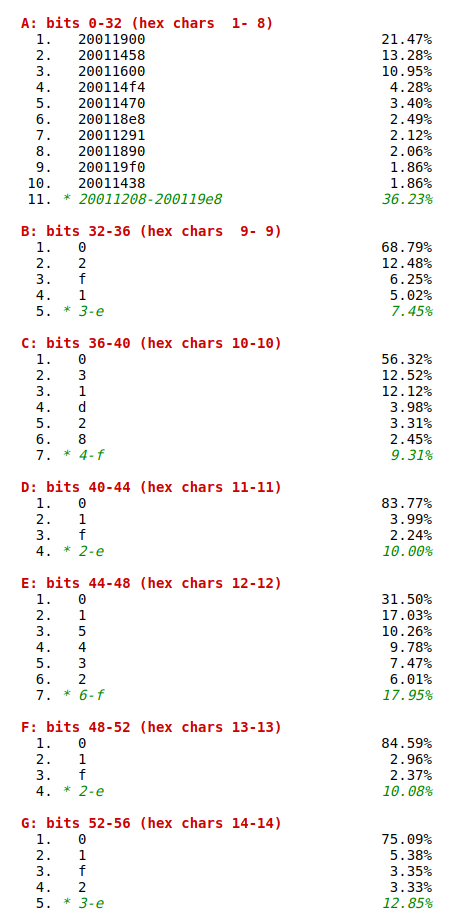
\includegraphics[width=0.3\textwidth]{dbscan}
\caption{DBSCAN}
\label{fig:dbscan}
\end{figure}

\section{贝叶斯网络}

将 IPv6 地址表示为随机向量, 我们可以很容易应用常见的统计模型. 我们选择使用贝叶斯网络来对 IPv6 地址段进行关联性分析.

贝叶斯网络是一种以有向无环图的形式表示联合分布随机变量的统计模型, 每个顶点代表一个变量, 从顶点 X 到顶点 Y 的一条边表示 Y 在统计上依赖于 X. 贝叶斯网络可以用来模拟包含许多变量的复杂对象, 将其分割为相互关联的小对象.

我们使用 BNFinder 程序构建 IPv6 地址的贝叶斯网络. 为了降低复杂度, 我们对网络进行约束: 每段只能依赖其之前的段. 我们将 IPv6 地址重新编码并于依赖性约束一起传递给 BNFinder 程序, BNFinder 程序运行后得到一个 cpd 文件, 其中存储了段间的关联性及具体的概率. 基于该文件, 我们可以依概率生成 IPv6 地址.

图~\ref{fig:bayes}~展示了样本集的贝叶斯网络.

\begin{figure}[htbp]
\centering
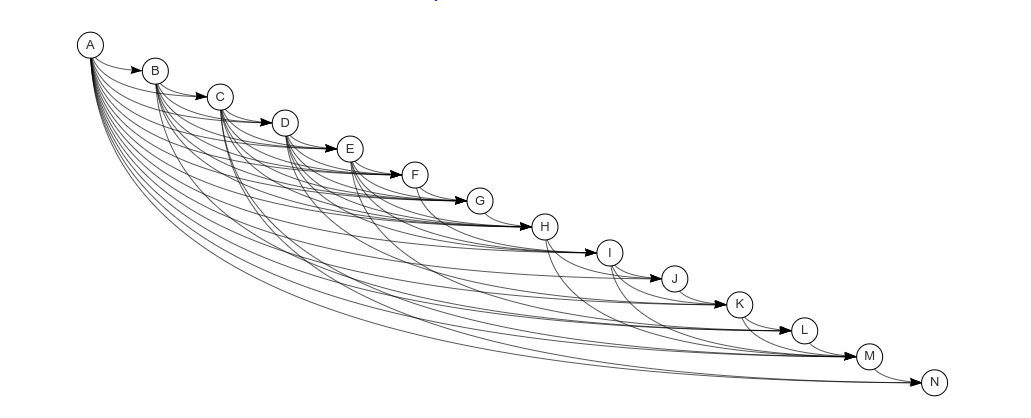
\includegraphics[width=0.6\textwidth]{bayes}
\caption{贝叶斯网络}
\label{fig:bayes}
\end{figure}
